\section{Demographic}
\label{demographic}

\subsection{Respondent's Age}
Age of a person often determines his/her knowledge and experience with the focus of the survey. When administering a survey about SE industries, a respondent in his 24s and 25s will most likely answer the question differently than a respondent his 35s. The age distribution of our survey respondents is shown in \cref{fig:age}.
\begin{figure}[H]
\centering
  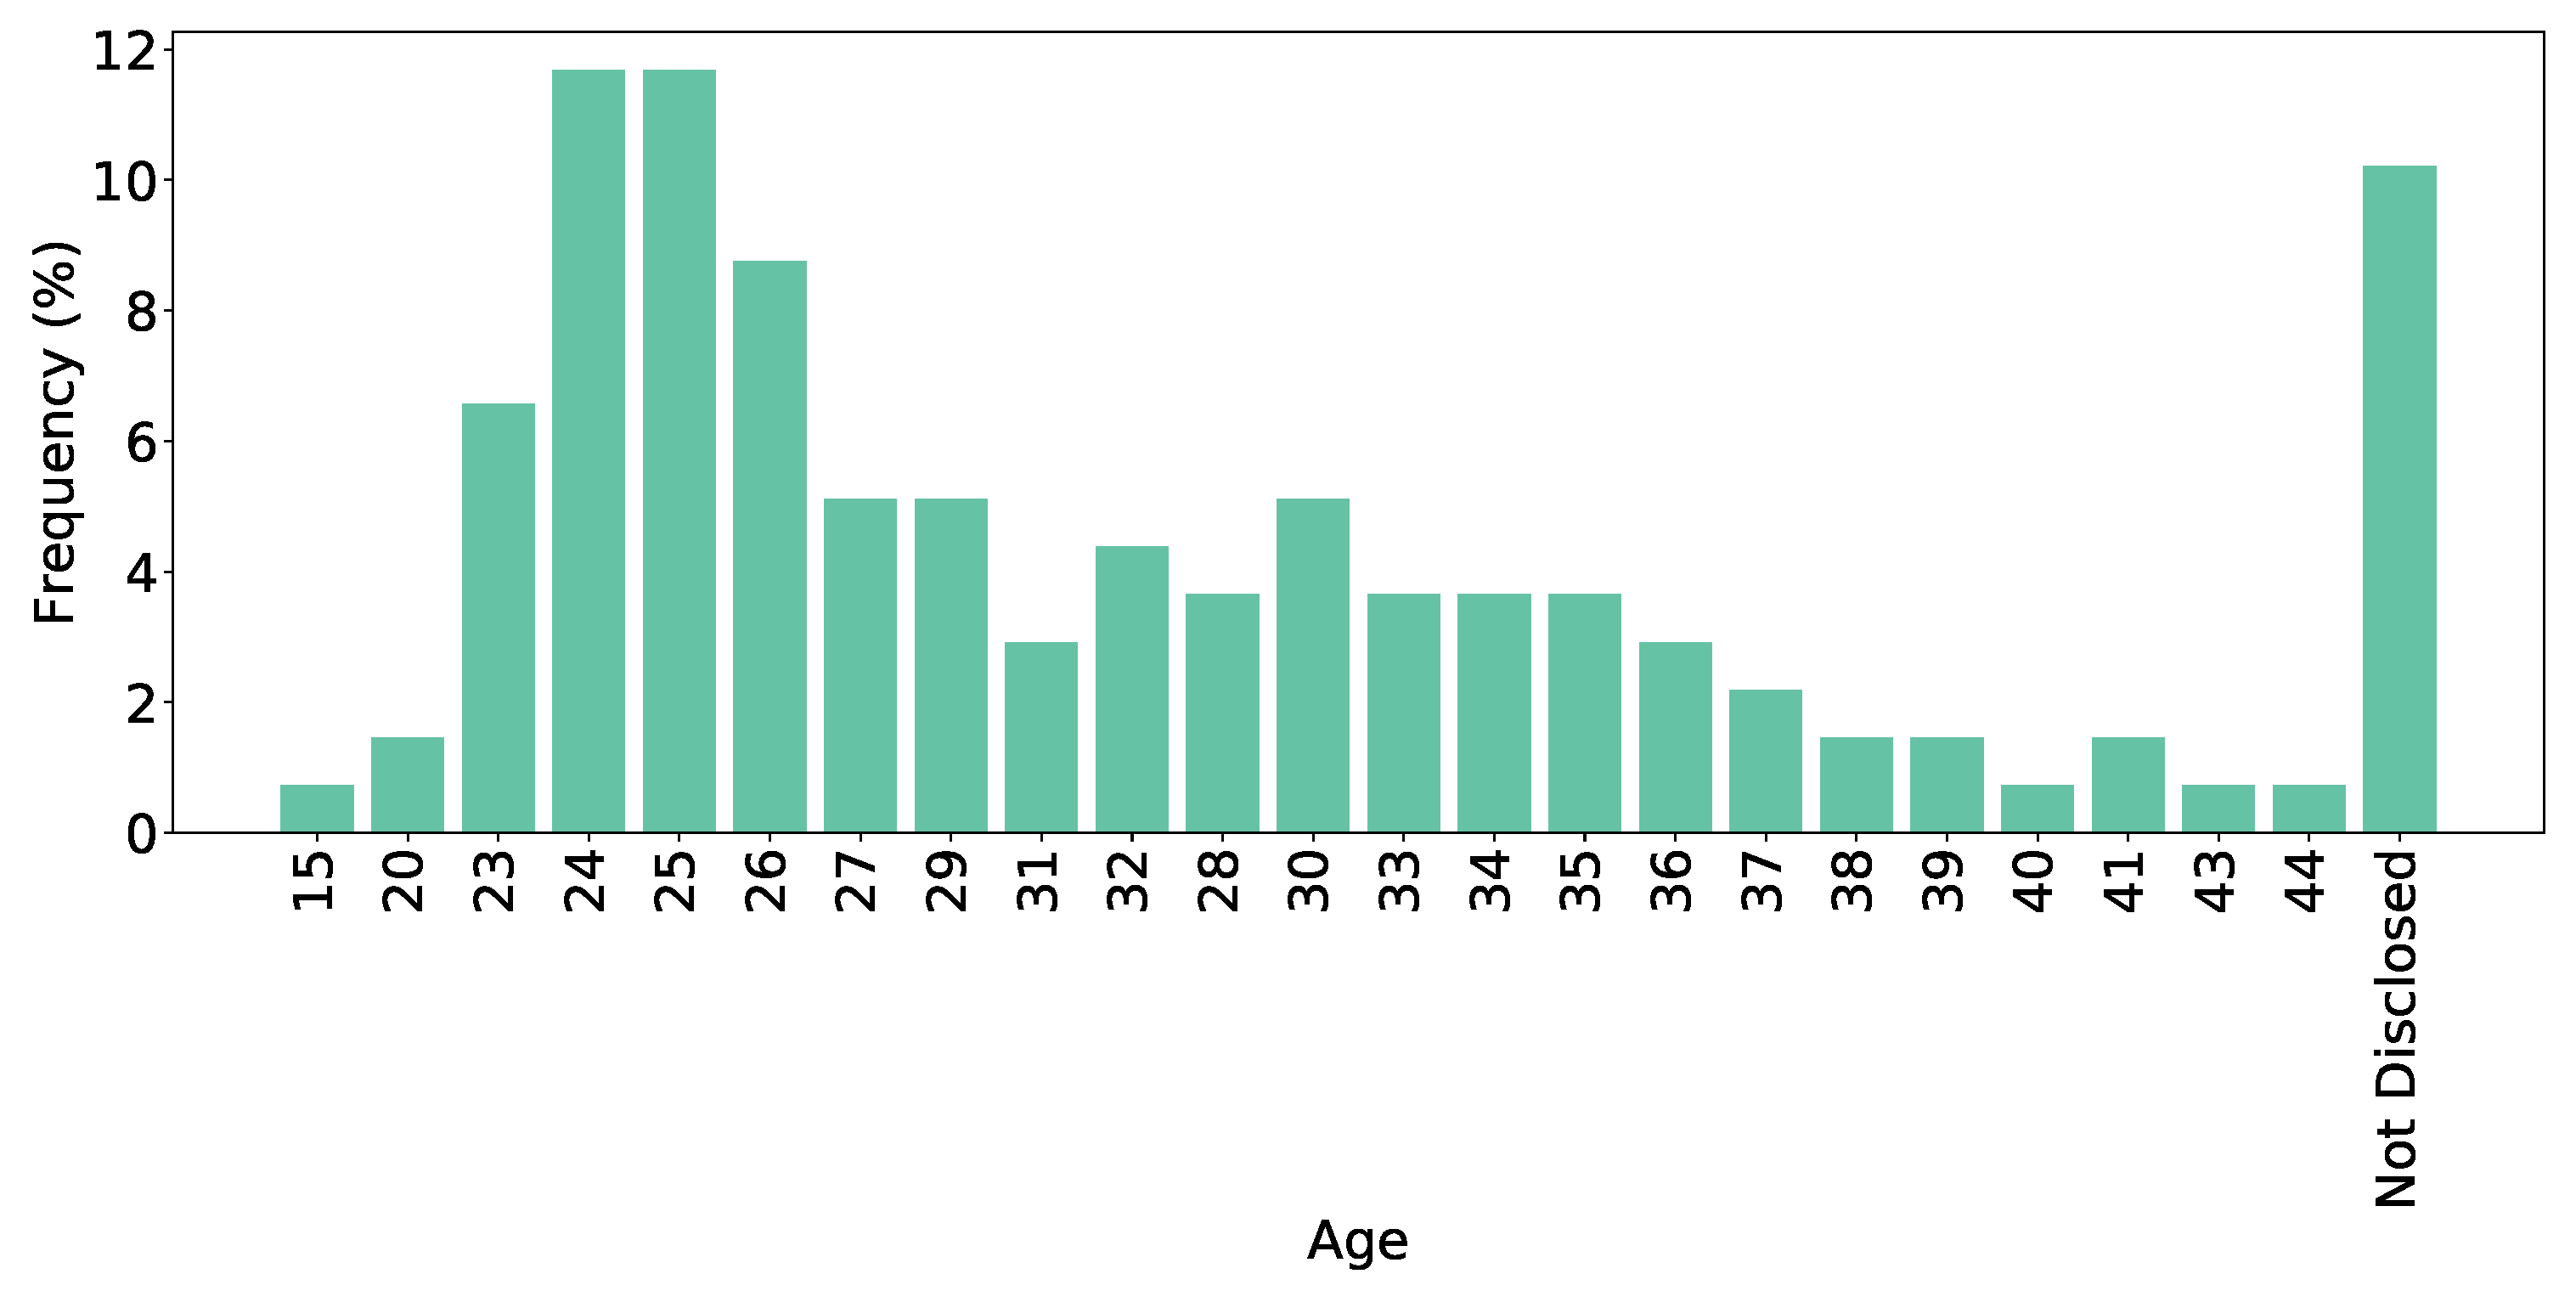
\includegraphics[width=0.8\textwidth]{Figures/Respondents_Age}
  \caption{Respondent's Age}
  \label{fig:age}
\end{figure}

\subsection{Work Experience}
Around 34\% of our respondent's has less than 2 years software development experiences. As the \cref{fig:experience} shows, we have respondent's with various years of work experience which will have positive impact by accumulating valuable results from wider audience base.
\begin{figure}[H]
\centering
  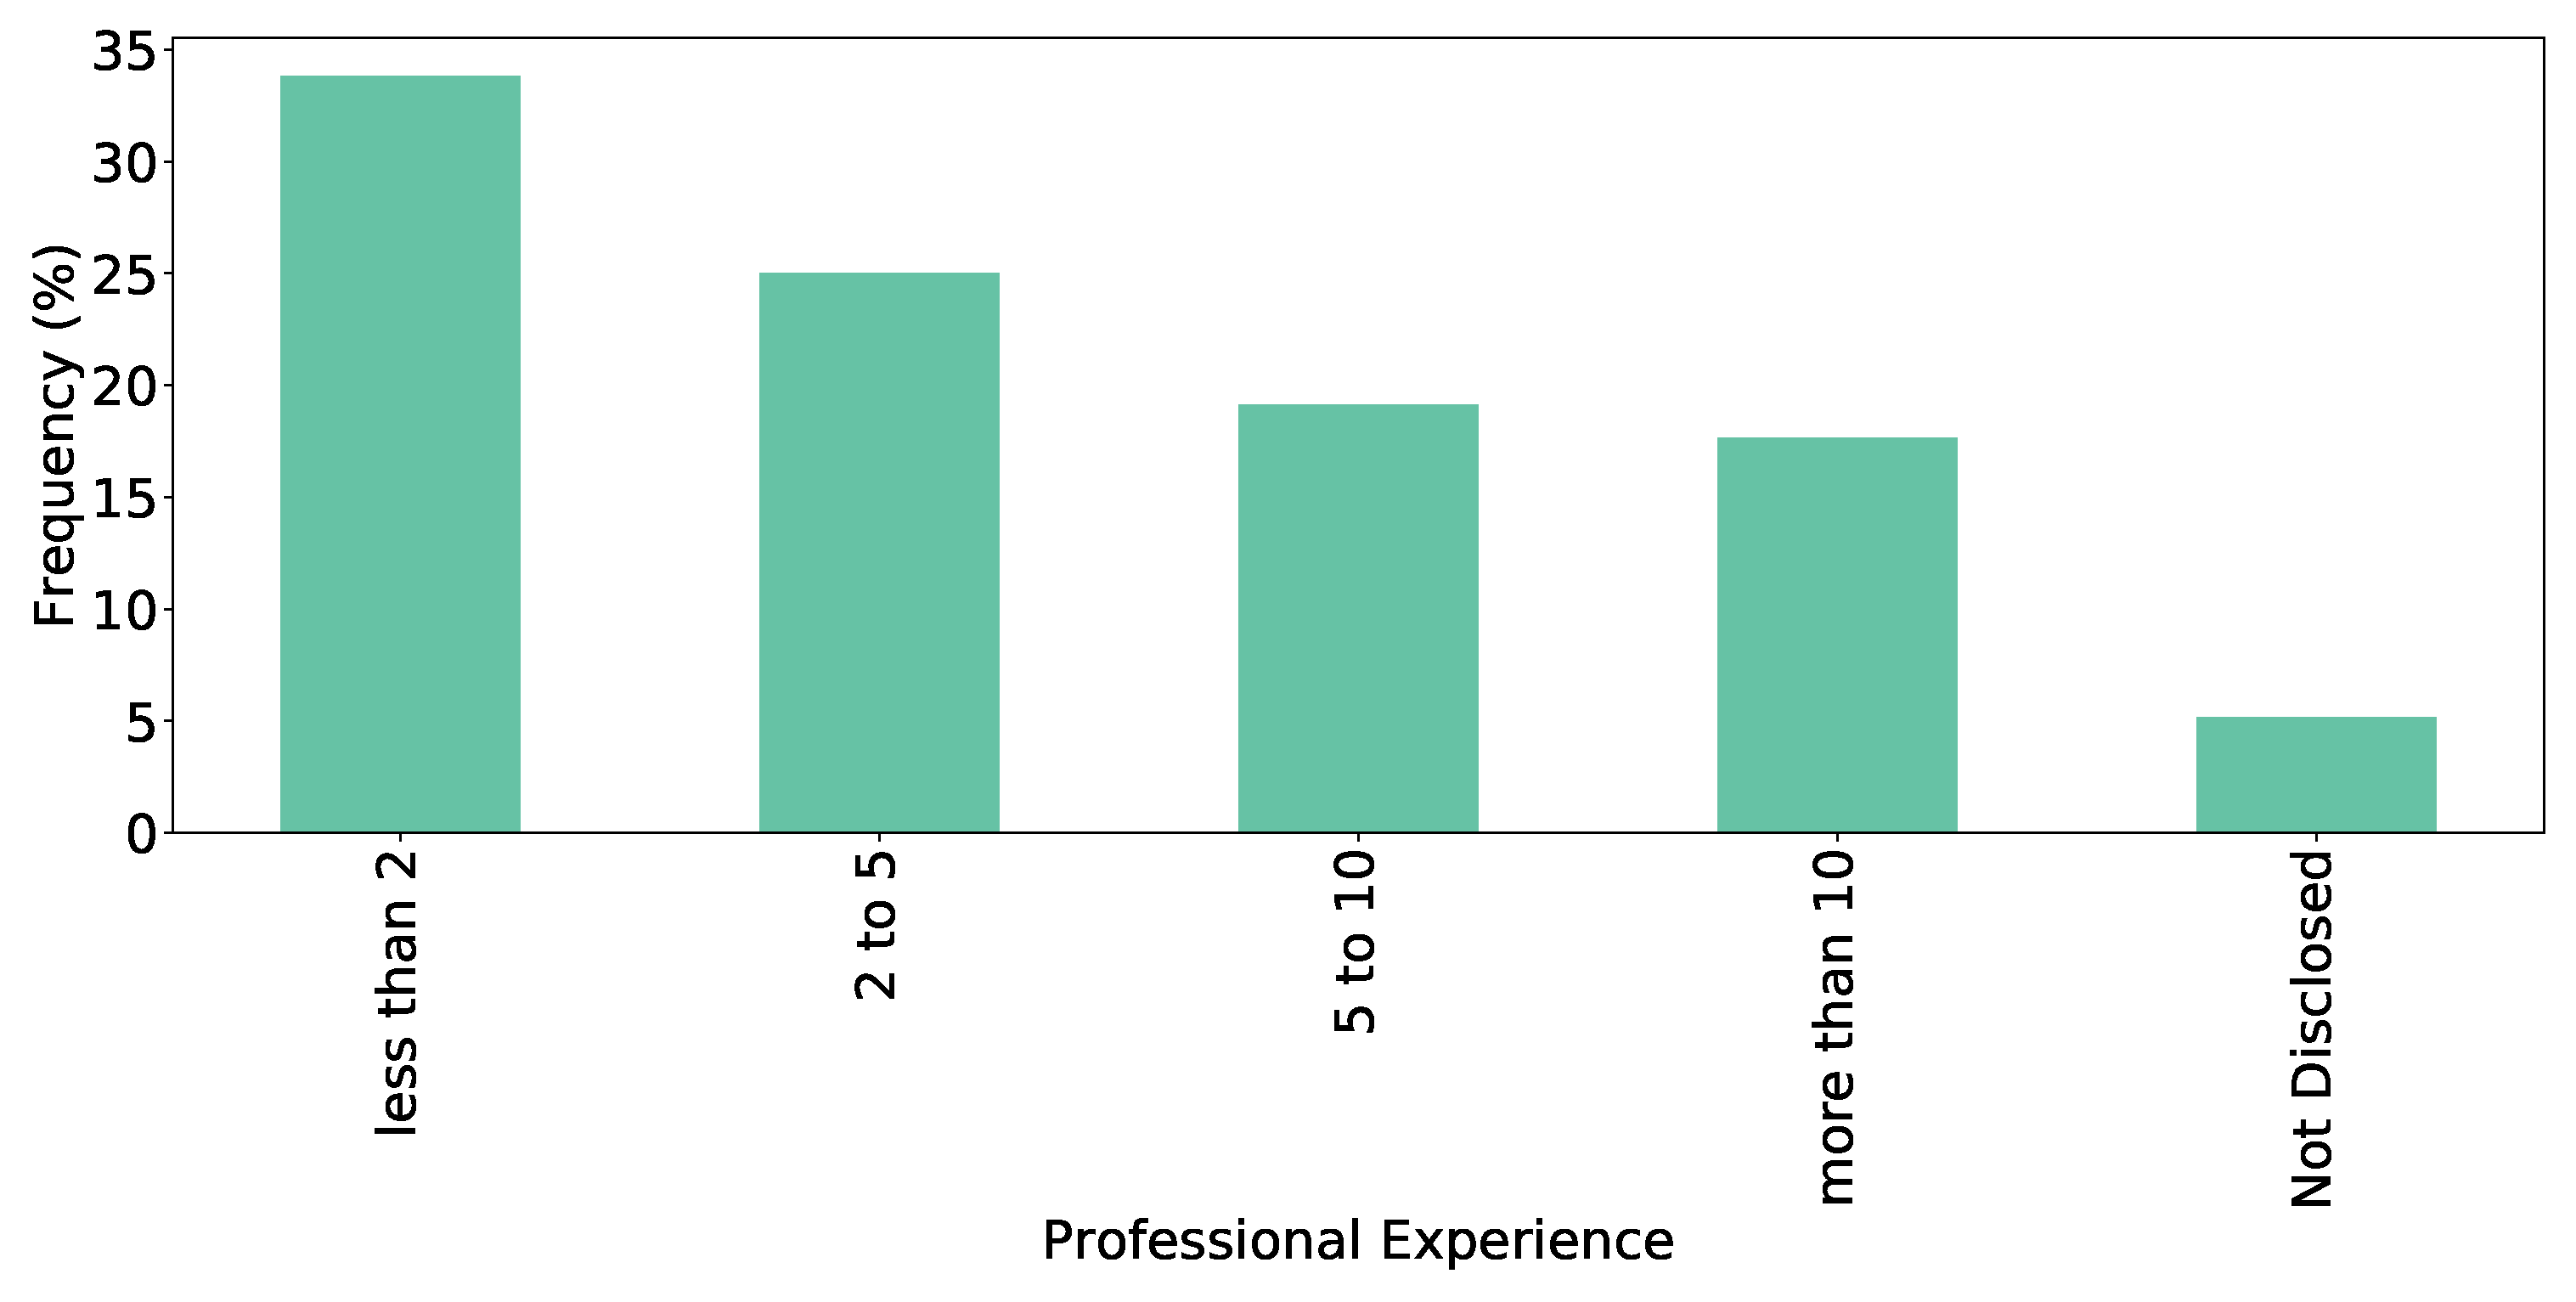
\includegraphics[width=0.8\textwidth]{Figures/Respondents_Experience}
  \caption{Work Experience}
  \label{fig:experience}
\end{figure}

\subsection{Respondent's Current Role}
From the \cref{fig:role} we see most of the respondents (70\%) were software developers and approximately 18\% of our respondent's are working at manager level post which have appreciable impact on getting expectations from managers.
\begin{figure}[H]
\centering
  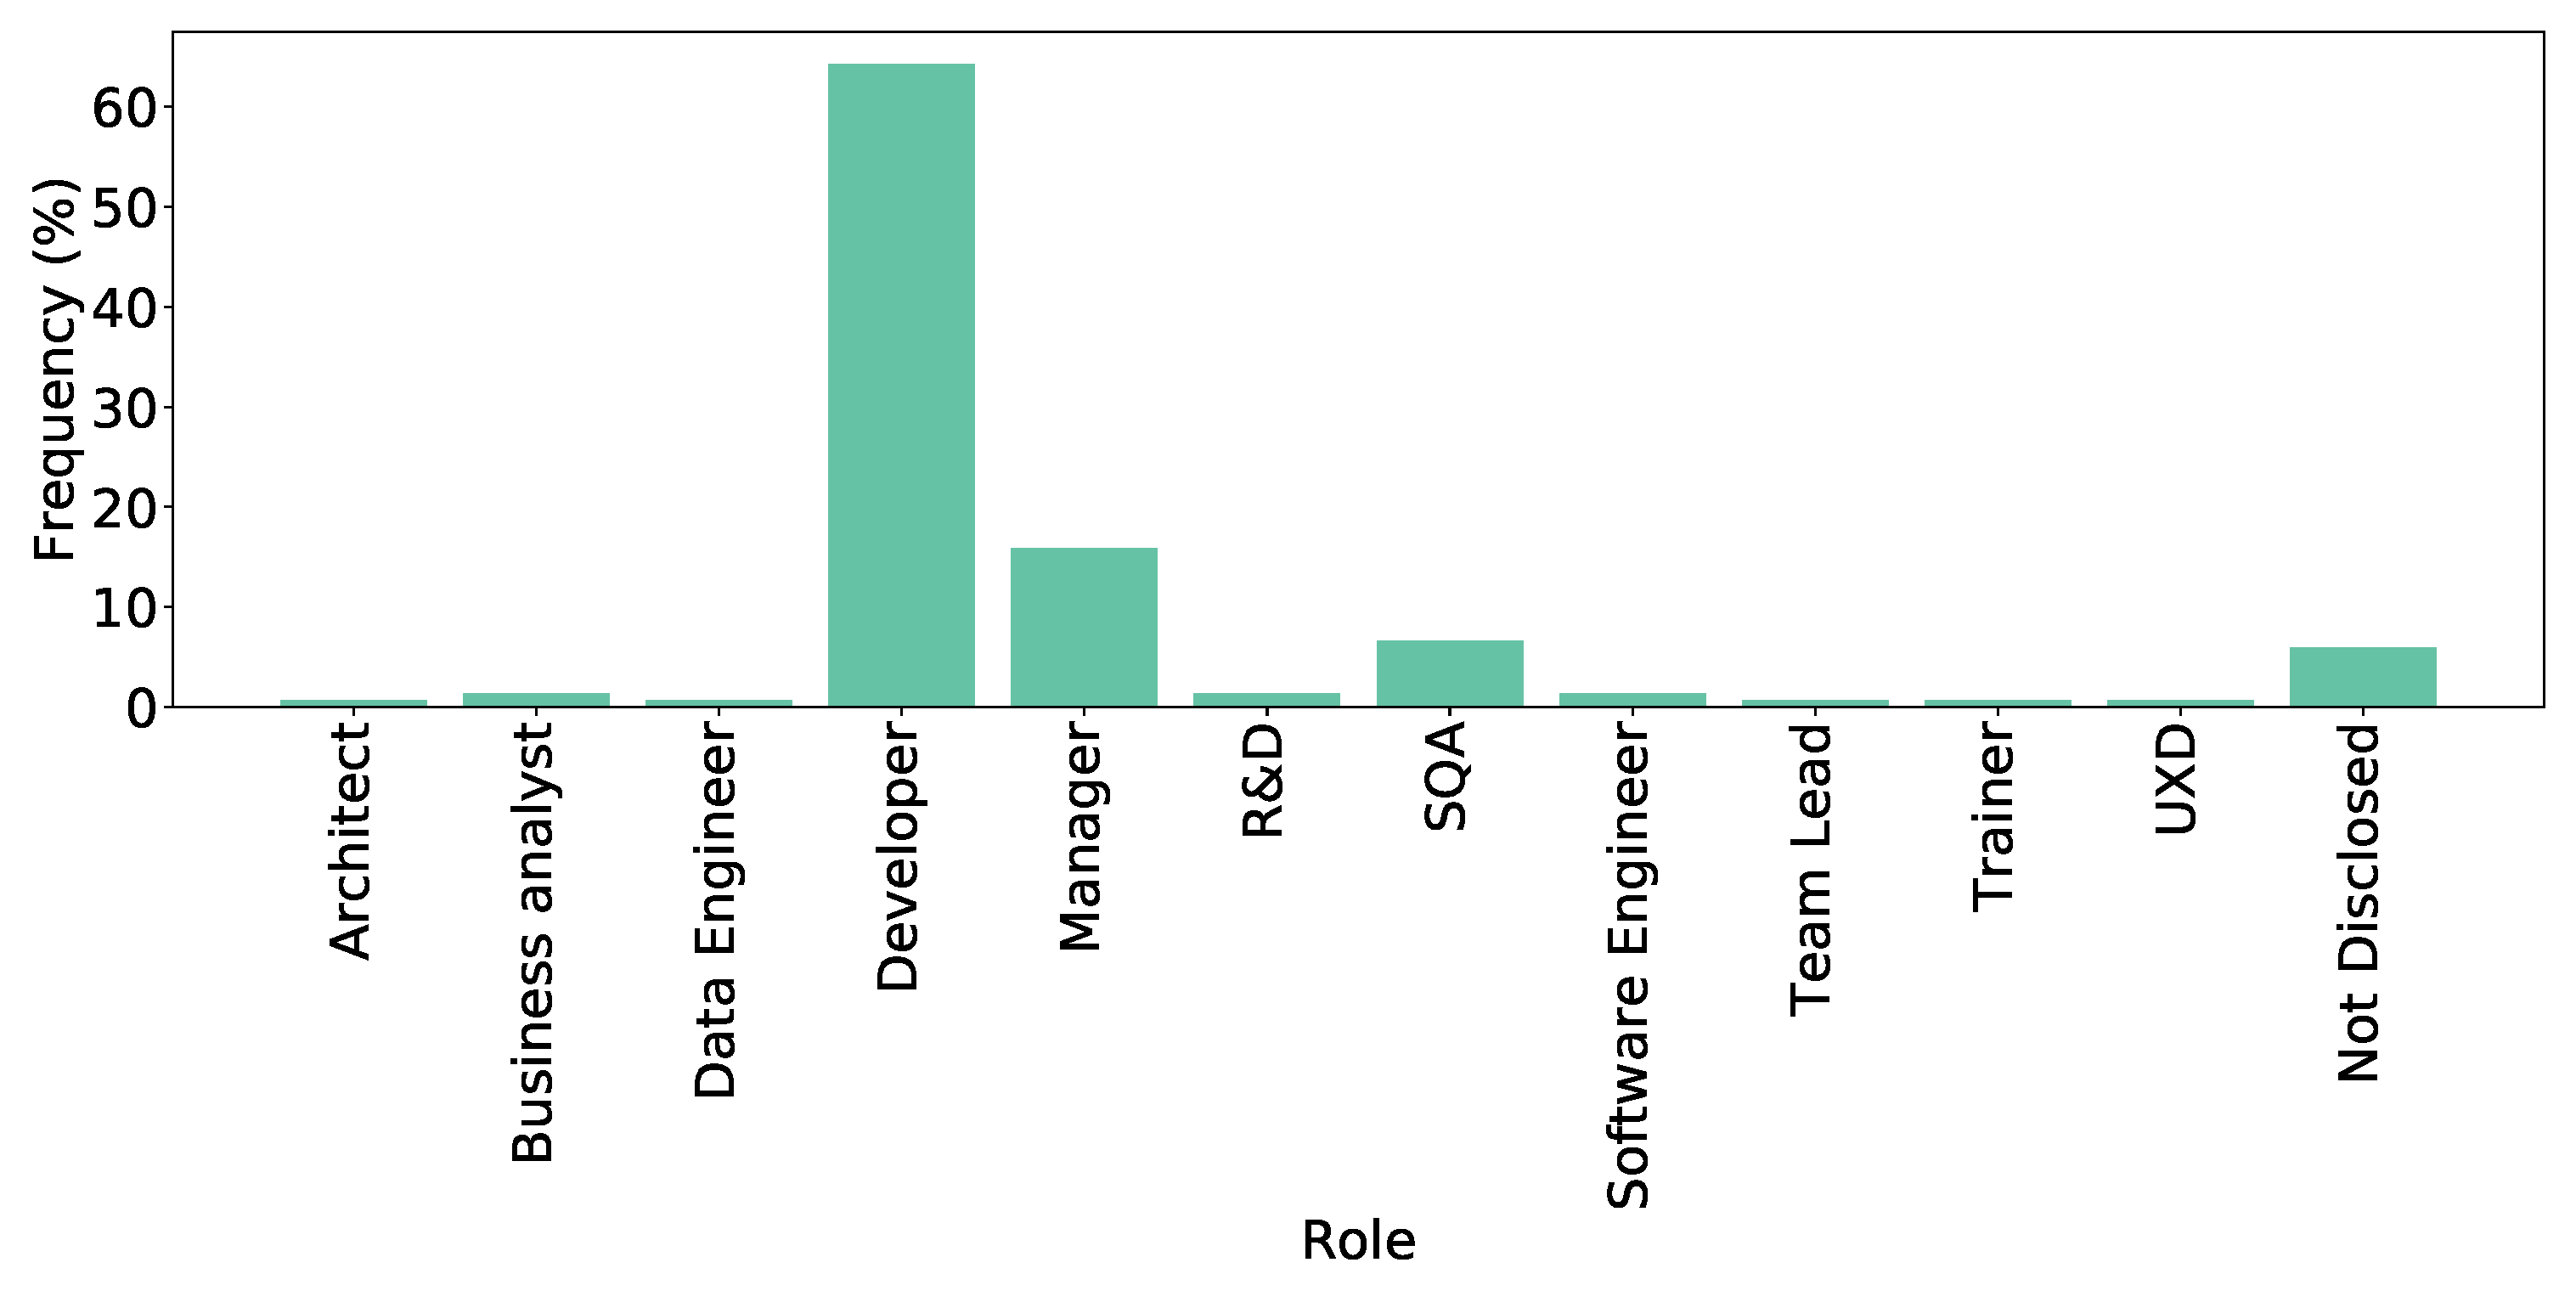
\includegraphics[width=0.8\textwidth]{Figures/Respondents_Role}
  \caption{Respondent's Current Role}
  \label{fig:role}
\end{figure}